\section{Úvod}

% TODO WRITER: text

Zde vysvětlit problémovou situaci a otázky, které se budou v bakalářské/diplomové práci řešit.

\section{Cíl práce}

% TODO WRITER: text

Smysl a účel, výzkumné otázky.

%teoretická část
\section{Metodika zpracování}

% TODO WRITER: text

Cíle, hypotézy/ výzkumné otázky, způsob hledání odpovědí na výzkumné otázky včetně metodiky vlastního výzkumu/šetření, literární rešerše.

\section{Úvod do problematiky Cyber-security}
%todo writer clean uvod?
V dnešní době díky rozvoji moderních technologií tráví velká část lidské populace značné množství času interakcemi s těmito tachnologiemi.
Ať už se jedná o Internet, \ac{IoT}, mobilní bankovnictví nebo sociální sítě, lidé se na technologií stávají čím dál více závislí.
Technologie nám usnadňují všední život, dovolují práci z domova nebo přináší příležitosti, které jen pár let předem neexistovaly.
Tento rozvoj bohužel není jen kladný.
Rozvoj se projevil i hrozbami, kterým populace čelí.
Některé hrozby, jako malware jsou pro lidstvo nové.
Jiné jsou staré jako lidstvo samo a pouze se novým okolnostem přizpůsobily.
Jedním příkladem za všechny je Sociální inženýrství.

\paragraph{}
Hrozbám nečelí jen samotní lidé ale i firmy a dokonce státy.
Státy na celém světě se staly na cybernetickém světe zcela závislé.\cite{LI20218176}
Jakékoli jeho selhání může ohrozit jejich funkčnost a odvázání se od něj je již nemožné.
Existuje nezměrné množství hrozeb.
Je jasné, že v prostředí kde mezi sebou soupeří státy je značné úsilí věnováno jak zabezpečení tak útoku.
Rozdíly mezi cyber-útokem, cyber-zločinem a cyber-válkou jsou ve většině případů rozděleny pouze dle účastníků.\cite{LI20218176}
Způsob útoku či hrozby na zatřídění do předchozích kategorií klade minimální vliv, zohledněn bývá pouze výsledek.

\paragraph{}





\subsection{Relevance}
Relevantnost problematiky cyber-bezpečnosti potvrzuje nejen množství akademických textů které zkoumají tuto problematiku, ale také stále větší zájem všeobecné veřejnosti.
Hlavním důvodem je vzrůstající povědomí populace, způsobené medializací útoků sociálního inženýrství nebo ransomware které populaci v poslední době ovlivňovaly.
V době psaní je v popředí například ransomware útok na dětskou nemocnici SickKids.\cite{bleep_sickkids_ransom}
I když Ransomware skupina \textit{LockBit} poskytla nemocnici \textit{decryptor} zdarma a s omluvou, nemění to nic na vážnosti situace.
Je totiž důležité si uvědomit, že takovýto útok nastal.
Byl schopen omezit optimální funkčnost nemocnice zašifrováním důležitých interních systému.
A bohužel není jediným ransomware útokem zaměřeným na zdravotnictví.
Je tedy možné předpokládat, že nastanou i další útoky na nemocnice.
A příští útok nemusí být veden skupinou, která se řídí silným morálním kompasem.
Důležité je na závěr poznamenat, že tento silný morální kompas platí jen na omezení funkčnosti které může vést ke smrti.
Nevztahuje se na méně kritické instituce nebo ani na prodej již získaných zdravotních dat na černém trhu.

\paragraph{}
Je tedy důležité věnovat se i nadále cyber-bezpečnosti.
Jsou hrozby, které jsou dobře prostudované a víme, jak se jim efektivně bránit.
Jsou hrozby, kterým je sice obtížné se bránit, ale jsou omezené rozsahem a tak je obrana uskutečnitelné.
Ale také jsou hrozby, na které obrana zatím neexistuje.
Tyto hrozby je nutné najít a zkoumat, aby bylo možné ochranu vytvořit.

\subsection{Studie trendů Cyber-security}
Dlouhodobě můžeme v rámci Cyber-security rozeznávat několik klíčových zaměření.
Zajímavé jsou změny v prioritách zaměření v ohledu na čas, které můžeme zkoumat na literatuře.
Velké změny lze zaznamenat především před a po pandemii Covidu-19.\cite{KUMAR2022102821}
Jako i u jiných odvětví můžeme dělit celou sféru na 2 části, část akademickou a část veřejnou.
Je jasné, že zaměření těchto dvou částí budou lehce rozdílná, proto je nutné dívat se na ně odděleně i když se v mnoha ohledech překrývají a ovlivňují.
Důvod proč zkoumáme rozdíl před a po Covidu-19 je rapidní navýšení adopce digitálních technologií, které v této době proběhlo.
Ztížené pracovní podmínky vyžadovaly zavádění nových technologií.
To znamená nová bezpečnostní rizika vzniklá nejen z těchto technologií, ale i z přístupu jejich využívání.
Je značný rozdíl v bezpečnosti práce uživatele, nachází-li se v uzavřené síti uvnitř společnosti nebo při připojování na dálku při práci z domova.

\paragraph{Akademická literatura}
V akademické sféře je možné vidět zaměření výzkumu.
Dlouhodobě populárními tématy jsou jsou \textit{cyber risk management, detekce malware} nebo \textit{systémy detekce přístupu}.\cite{KUMAR2022102821}
Tato témata je možné nalézt jak před, tak i po pandemii Covidu-19.
Témata, které byla mnohem více zkoumána před pandemií jsou například využití \textit{Machine learningu}, a to jak pro detekci hrozeb tak hledání nových útočných vektorů.
Také \textit{Blockchain} a \textit{Crypměna} jsou témata, která byla před pandemií v oblasti zájmu akademiků mnohem více, nežli po pandemii.\cite{KUMAR2022102821}
Pandemie způsobila velký zvrat v myšlení.
Vedlo to ke zkoumání témat, které bylo nutné okamžitě aplikovat nebo která byla nutné pro budoucí fungování společnosti.
Objevují se zde mnohem více témata zaměřená na \textit{Zdravotnictví, Bankovní sektor} nebo \textit{zranitelnosti dodavatelského řetězce}.\cite{KUMAR2022102821}
Všechna tato témata mají jasný vznik v okolnostech pandemie a jejich zkoumání je prováděno i roky po pandemii samotné.

\paragraph{Všeobecná literatura}
Všeobecná literatura poukazuje na zájmy a zvědavost lidu, proto zde lze odvodit zaměření ale také problémy populace.
Před pandemií byly nejčastější témata zaměřená na \textit{finančně zaměřené cybernetické útoky}.
Ty spolu s běžnými tématy jako \textit{běžné bezpečnostní slabiny, úniky dat} a \textit{malware incidenty} vzbuzovaly největší zájem médií.\cite{KUMAR2022102821}
Pandemie rapidně změnila zájem lidu.
Zaměření se přesunulo na útoky, které se během pandemie značně rozšířily.
Jsou jimi hlavně \textit{Sociální inženýrství} nebo útoky \textit{ransomware}.
Také útoky na \textit{Zdravotnictví} byli mnohem častěji reportovány medii.
Tématem, které je v obou obdobích významné je \textit{malware}.
Jeho primární zaměření se však liší.
Před pandemií byla literatura zaměřena hlavně na ovlivnění správného chodu firem.
Po pandemii se psalo spíše o dopadech na digitální infrastrukturu jako jsou \textit{služby v cloudu}.

\subsection{Nejčastější útoky}
% TODO WRITER: text?

tohle je reference na obrázek \ref{MostCommonAttacks}.

\begin{figure}{\linewidth}
	\centering
	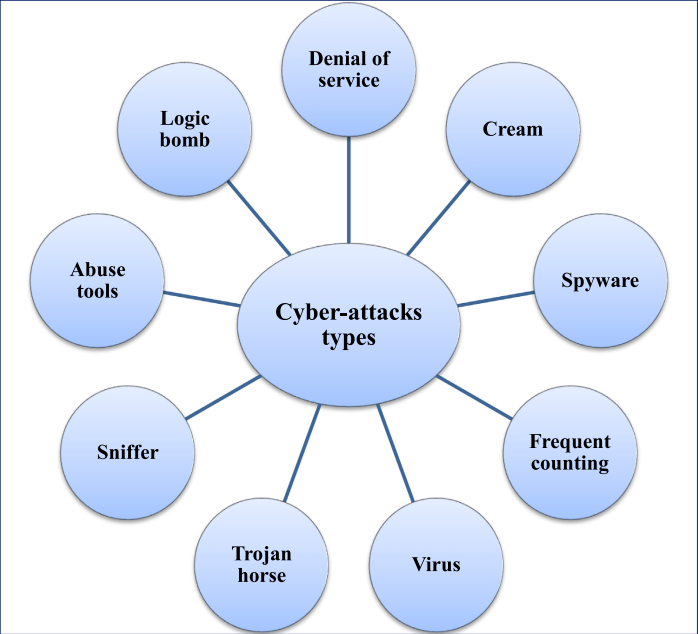
\includegraphics[width=\linewidth]{Images/cyber_attack_types}
	\caption{Nejčastější typy cyber-útoků}
	\label{fig:MostCommonAttacks}
\end{figure}



% TODO WRITER: text?

\subsection{Testování}
Pro zlepšení bezpečnosti jsou doporučovány 3 hlavní testovací metodologie: Penetration testing, Red team assessment a Purple team/kontrolní cvičení.
Z důvodu přesahu vlastností jsou tyto metodologie zaměňovány, někdy dokonce považovány za jedinou metodologie s několik různými názvy.\cite{securityInteligence_pen_test_red_team_purple_team}

\paragraph{}
Právě z těchto důvodů jsou v následujícím textu vysvětleny.

\subsubsection{Penetration testing}

Penetration testing, často také zkracován na pen testing, je metodologie s cílem vyhledání co nejvíce možných zranitelností testovaného systému.
Takto důkladné hledání je omezeno pouze na zadaný ,scope', neboli část testovaného systému.
Aby bylo dosaženo co největší efektivity, tento typ testování se svoji činnost nesnaží schovávat, naopak bývá velmi snadné ho detekovat, to však nevadí protože ochrana daného systému by o jeho provádění měla být předem informována.
Tento typ testování může být také z části automatizován, což vede k dalšímu zlepšení efektivnosti na úkor flexibilitě.
V neposlední řadě Penetration testing vyžaduje menší množství zdrojů, ať už v podobě času, lidí či kapitálu, než red team assessment.
\paragraph{}
Ve shrnutí, Penetration testing je hledání co nejvíce zranitelnosti v zadané oblasti bez nutnosti svoji činnost maskovat před ochranou systému.\cite{securityInteligence_pen_test_red_team_purple_team, lootsec_pen_test_vs_red_team, astra_pen_test_vs_red_teaming}


\subsubsection{Red team assessment}

Red team assessment, také referovaný jako red teaming, je na rozdíl od pen testingu zaměřen na dosažení zadaných cílů, například získání přístupu k citlivým datům, nebo testování všímavosti ochranných systémů.
To také znamená, že red teaming není omezen oblastí, kterou může v rámci dosažení svého cíle využít.
Obrana systému není ze zřejmých důvodů seznámena s nadcházejícím testováním, proto tato metodika vyžaduje maskování a opatrný přístup, aby pokud možno co nejvíce simulovala skutečný útok.
Výhodou je, že za předpokladu detekce testování bude obrana systému postupovat stejně, jako kdyby se jednalo o skutečnou hrozbu a získáme tak cenná data a zpětnou vazbu pro zlepšení budoucí obrany.
Je jasné, že pro správné provedení red teamingu je potřeba více zdrojů, at už se jedná o čas nebo lidskou práci, než v případě pen testingu.
Také automatizace zde bývá složitá, jedná se totiž o specifickou strategii pro každé testování kde je nutnost reagovat na všechny události vzniklé testováním.\cite{securityInteligence_pen_test_red_team_purple_team, lootsec_pen_test_vs_red_team, astra_pen_test_vs_red_teaming}

\paragraph{}
Ve shrnutí, red team assessment je zaměřen na testování obranyschopnosti cíle s omezeními vznikajícími pouze ze snahy simulovat reálný útok.

%todo use this resource
todo\cite{red_team_oakley_2019}

\subsubsection{Purple team/Kontrolní cvičení}
Specifická situace je pak blízká spolupráce útočníků (Red team) a obránců (Blue Team).
Hlavní výhodou tohoto postupu je zpětná vazba mezi útočníky a obránci, kde se dá testovat detekce a následná odezva obránců při testování specifických technik obsažených v MITRE ATT\&CK frameworku.
Další výhodou je seznámení s postupy druhé strany pro tvorbu efektivnějším strategií, at už se jedná o útočníky nebo obránce.
\paragraph{}
Tato cvičení lze uskutečňovat pouze jednou pro vyzkoušení techniky nebo také opakovaně.
Částečná automatizace za použití open-source nástrojů, které mají v této práci vlastní kapitolu, je také jednou z možností.
Výhodou opakovaného testování s automatizací je možnost měřit a porovnávat výsledky za stejných stupních podmínek, což vede k jasně viditelnému zlepšení obranné strategie.\cite{securityInteligence_pen_test_red_team_purple_team,redscan_team_purple_team}

\subsection{Zavedené nástroje v problematice Testování}

ATT\&CK a red teamy, caldera
atomic red team, co má za nároky, atd atd, udělat porovnání s caldera atd

% TODO WRITER: text


kouknout co se v problematice řeší, ukázat klady a zápory (ideálně 2 stránky do vánoc)

\subsubsection{Mitre ATT\&CK}
% TODO WRITER: text
vysvětlit matici, co nám přináší

\subsubsection{Nástroje}
% TODO WRITER: text

udělat porovnání vybraných nástrojů(viz článek -> atomic red team, mitre caldera,..)
vlastní subsekce pro nástroje
MITRE Caldera, Uber Metta, Atomic Red Team and Endgame RTA

\subsubsection{Atomic Red Team}
% TODO WRITER: text
co to je, porovnání

\subsubsection{Mitre Caldera}
% TODO WRITER: text
co to je, porovnání


\section{Praktická část}

% TODO WRITER: text

\section{Závěry a doporučení}

% TODO WRITER: text

Kritická diskuze nad výsledky, ke kterým autor dospěl (soulad výsledků  literaturou či předpoklady;
výsledky a okolnosti, které zvláště ovlivnily předkládanou práci atd.).
Je vhodné naznačit i případné další
(popř. alternativní) možnosti zkoumání dané problematiky a otevřené problémy pro další studium.

% todo del - this is example and testing section

Vlastní řešení dokládá student zpravidla v několika kapitolách.
Podle charakteru práce musí student uvážit, zda informace
netextové povahy (data, tabulky, obrázky atd.) bude uvádět přímo v textu, nebo je zařadí až za celou práci ve formě příloh, či bude kombinovat oba způsoby.
Více podrobností viz Metodické pokyny pro vypracování bakalářských a diplomových prací (zveřejňované formou výnosů děkana)
a v kurzu MES – Metodologický seminář.

	\subsection{Podkapitola}

	Text podkapitoly.

	Následuje ukázka nějakého seznamu:
	\begin{itemize}
		\item fotografie/avatar,
		\item kategorizační štítky,
		\item popisek.
	\end{itemize}

		\subsubsection{Podpodkapitola}

		Lorem ipsum dolor sit amet, consectetur adipiscing elit. Phasellus sit amet ornare diam, id consequat diam.

			\nlparagraph{Paragraf}

			\noindent Ukázka prvního odstavce v paragrafu. Lorem ipsum dolor sit amet, consectetur adipiscing elit. Phasellus sit amet ornare diam, id consequat diam.


			Použití zkratek se rozděluje na první použítí a další použití: první použití \firstac{URL} a další použítí \ac{URL}.

			Použití obrázku je jednoduché, zadáme název souboru, šířku, popisek a zdroj:~\cntcapfigure{Images/rovnovaha_paka}{8cm}{Páka rovnováhy vzhledu.}

			V případně, že autor je i autor obrázku:

			\cntcapfigure{Image/uhk}{\linewidth}{Toto je UHK.}{[autor]}

			Blok kódu může vypadat takto:

			\begin{codeblock}
				\begin{verbatim}
@Mapper
public interface AccountDao {
  @Select({
    "select *",
    "from " + Account.TABLE_NAME,
    "where email = #{email}"
  })
  Optional<Account> findByEmail(String email);
}
				\end{verbatim}
				\captionsource{Ukázka bloku kódu.}{[autor]}
			\end{codeblock}

			Tabulka zas může vypadat takto:

			\begin{table}[hbt!]
				\captionsource{Ukázková tabulka.}{[autor]}
				\centering
				\begin{tabular}{| l | r | r | r | }
					\hline
					&        psnr &      ssim &      doba  \\
					model &       (db)    &           & gen. (s) \\
					\hline
					bik. int. & 28.3155 & 0.8566 & 0.0322 \\
					nn1000    & 30.1461 & 0.9043 & 0.8109 \\
					nn1001    & 30.0324 & 0.9023 & 0.7486 \\
					nn1002    & \textbf{30.1886} & \textbf{0.9046} & 1.1731 \\
					nn1003    & 30.0390 & 0.9030 & 1.1320 \\
					nn1004    & 24.9772 & 0.7172 & 4.4367 \\
					nn1005    & 26.1629 & 0.8004 & 4.0475 \\
					nn1006    & 27.9129 & 0.8438 & 4.0683 \\
					nn1007    & 27.5834 & 0.8360 & 4.2082 \\
					\hline
				\end{tabular}
			\end{table}

			\newpage

			Další text

\section{Závěry a doporučení}

% TODO WRITER: text

Kritická diskuze nad výsledky, ke kterým autor dospěl (soulad výsledků  literaturou či předpoklady;
výsledky a okolnosti, které zvláště ovlivnily předkládanou práci atd.). Je vhodné naznačit i případné další
(popř. alternativní) možnosti zkoumání dané problematiky a otevřené problémy pro další studium.
